\chapter{Mouse Behaviour in Complex VR Tasks}
\label{chapterlabel3}

\section{Can Mouse Learn Visually Complex Navigation Task?}
 Many recent studies in mouse VR navigation tasks use tall and large visual landmarks which can be seen and distinguished from far away with floor patterns as only background. In the experiment design I use, it presents the challenge to the mouse that it needs to differentiate sets of identical landmarks in grayscale and the well-controlled white noise gray background. Compared to primates, cats, birds, mice have low acuity vision. One may argue that mouse cannot differentiate such detailed visual landmarks in a VR setting to form clear representations of the space. In Saleem et al. 2018, they've trained the mice to actively lick for a reward associated to one of the identical plaid landmarks spaced at 20cm in a 100 cm corridor. Here in one of the environment, I use a familiar set of landmarks but with an additional cue landmark at the start with extension of extra 40 cm. Further to that, the VR corridor is constrained to only show 21cm ahead of the mouse rather than the full view ahead. This method prevents the mouse knowing what landmarks are ahead until it passes the current landmark and it is different from the conventional VR task particularly in studies on hippocampus and entorhinal cortices. Therefore, it can be perceptually more challenging to distinguish one visual landmark and 2 sets of identical visual landmarks in 100 cm space. In addition, in the recording period, there would be an extra environment introduced to the animal and the novel environment contains one of the same set of landmarks, that is, the plaids, and the mouse is required to distinguish the two environments are different. In this chapter, I will show mice can learn visually complex navigation tasks.

\section{Methods}






\section{Mice }

\begin{figure}
    \centering
    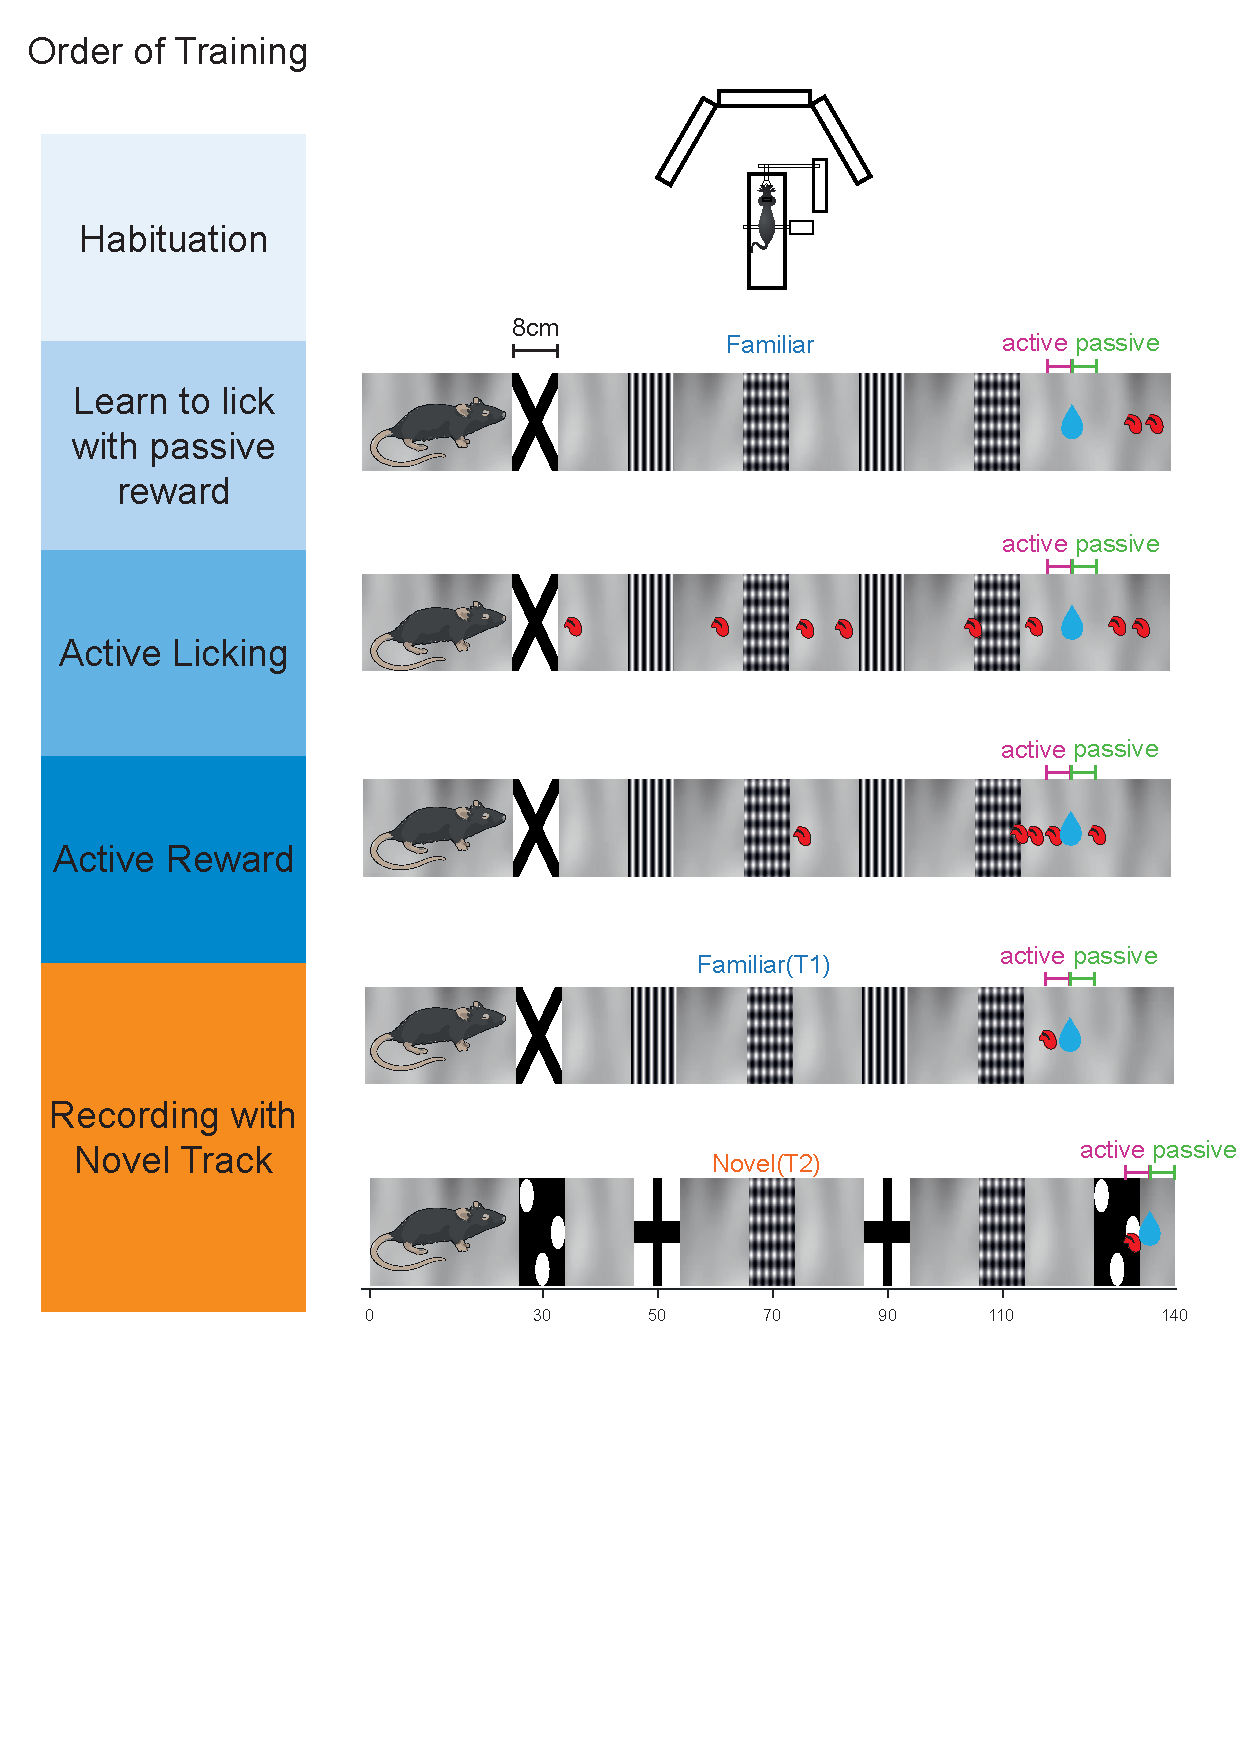
\includegraphics[width=1\linewidth]{figures//Chapter 3 Behaviour//Thesis Figures//figure_PDFs/fig1_behaviour_training.pdf}
    \caption{Training stages from habituation to recordings. }
\medskip
\small
The illustration gives examples of licking behaviour over stages of training. In early stage, the mouse can only lick after a passive reward is given. After habituation to the reward and licking, the mouse can lick actively everywhere in the VR. Once learned, the active licking is more likely to be around reward zone. Once the mouse is ready, it undergoes craniotomy surgery and the ephys recordings start with the introduction of novel VR environment.
    \label{fig:overall training stages}
\end{figure}





\begin{figure}
    \centering
    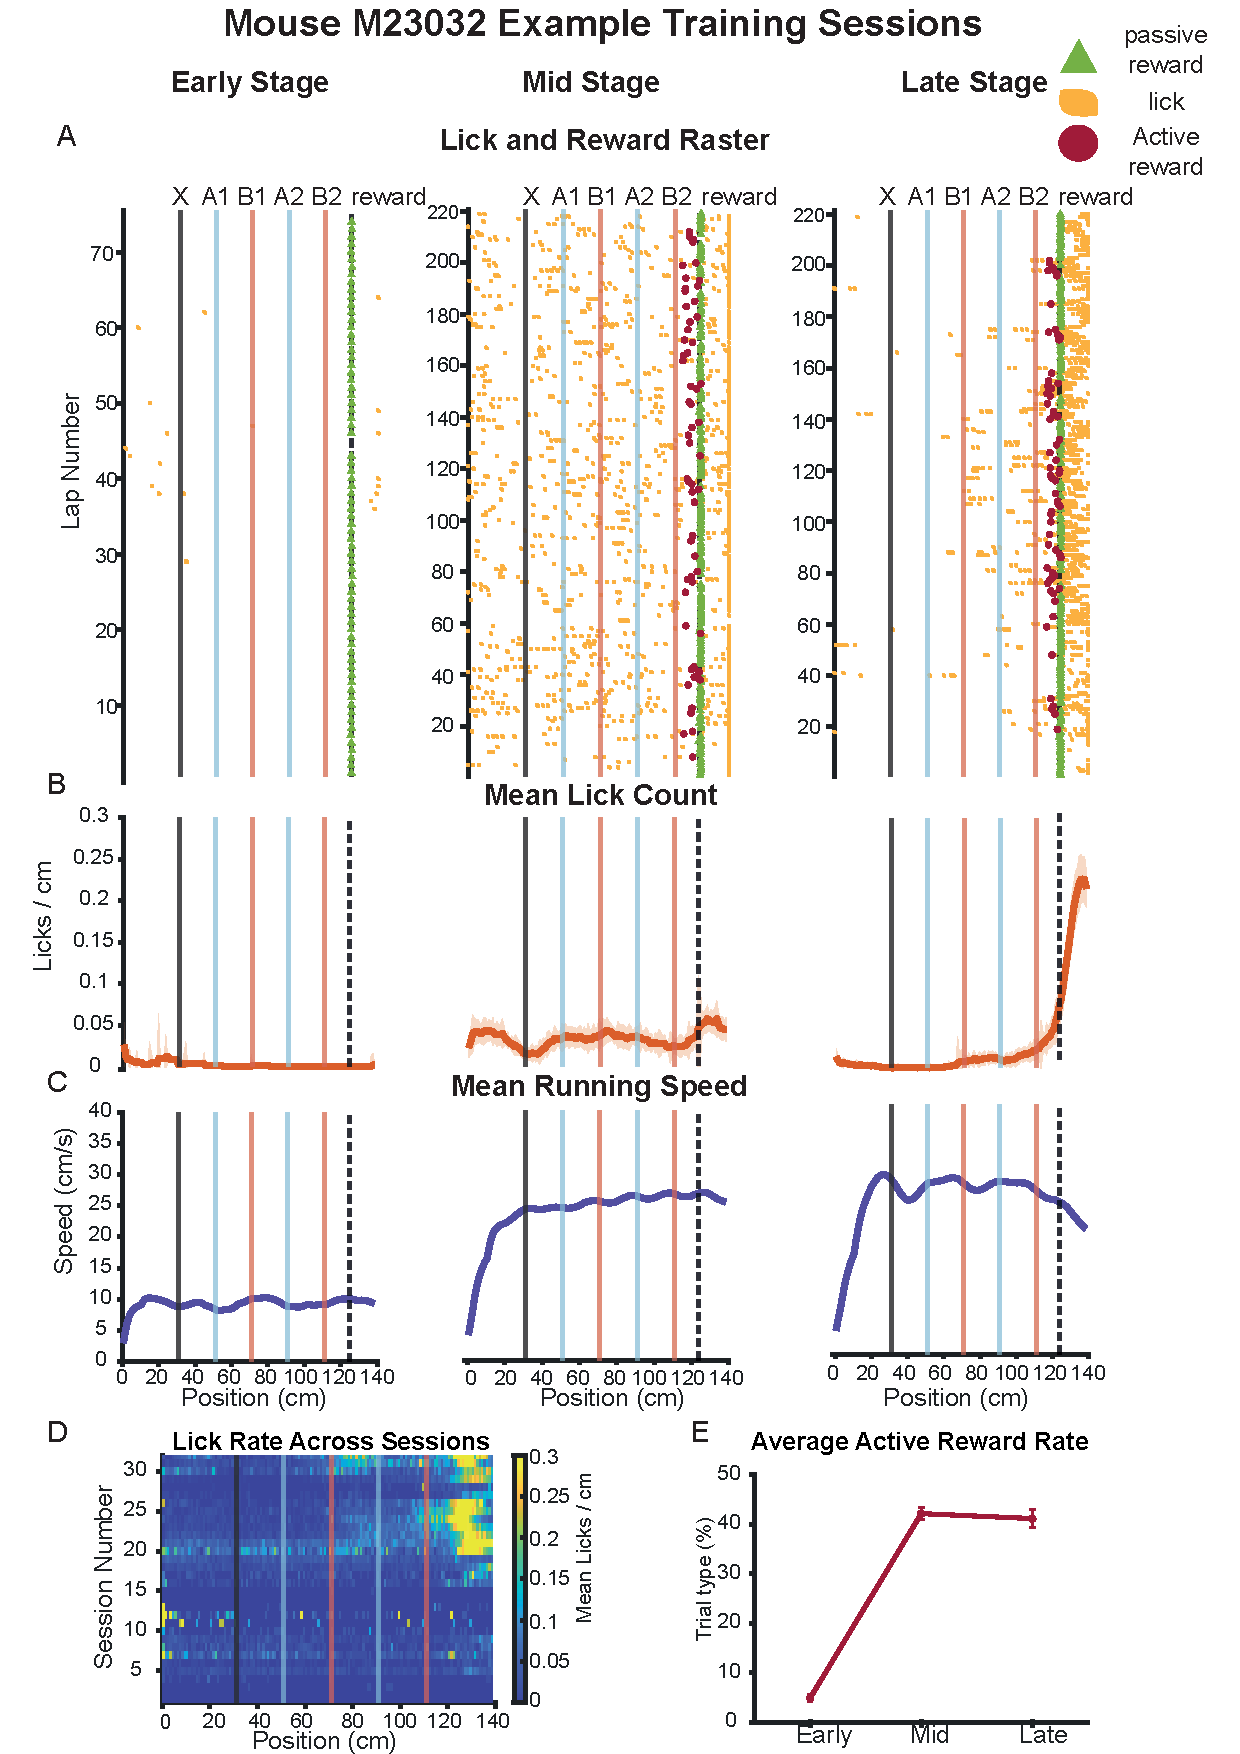
\includegraphics[width=1\linewidth]{figures//Chapter 3 Behaviour//Thesis Figures//figure_PDFs/fig2_example_sessions.pdf}
    \caption{Example training sessions at different stages of the training.}
\medskip
\small
 The three examples from mouse M23032 are each from early, mid, late stages of the training. \textbf{A)} Raster plots of licking, active rewards and passive rewards events. Green triangle is passive reward, yellow round object is mouse licking detected, red circle is active rewards. Y axis is the number of laps in the session and x axis is the position of the mouse. \textbf{B)} The average lick count at each position across laps in the session. Y axis is the mean lick count/cm and the x axis is the position. \textbf{C)} Average running speed at each position across laps in each session. The y axis is the speed (cm/s) and x axis is the position. \textbf{D)} The heatmap of overall mean lick count across sessions. Y axis is the session number and x axis is mouse position. The licking distribution slowly evolves into more active lickings around reward zone over learning. \textbf{E)} Average percentages of active reward in early, mid, late sessions. 
    \label{fig:example training sessions}
\end{figure}



\begin{figure}
    \centering
    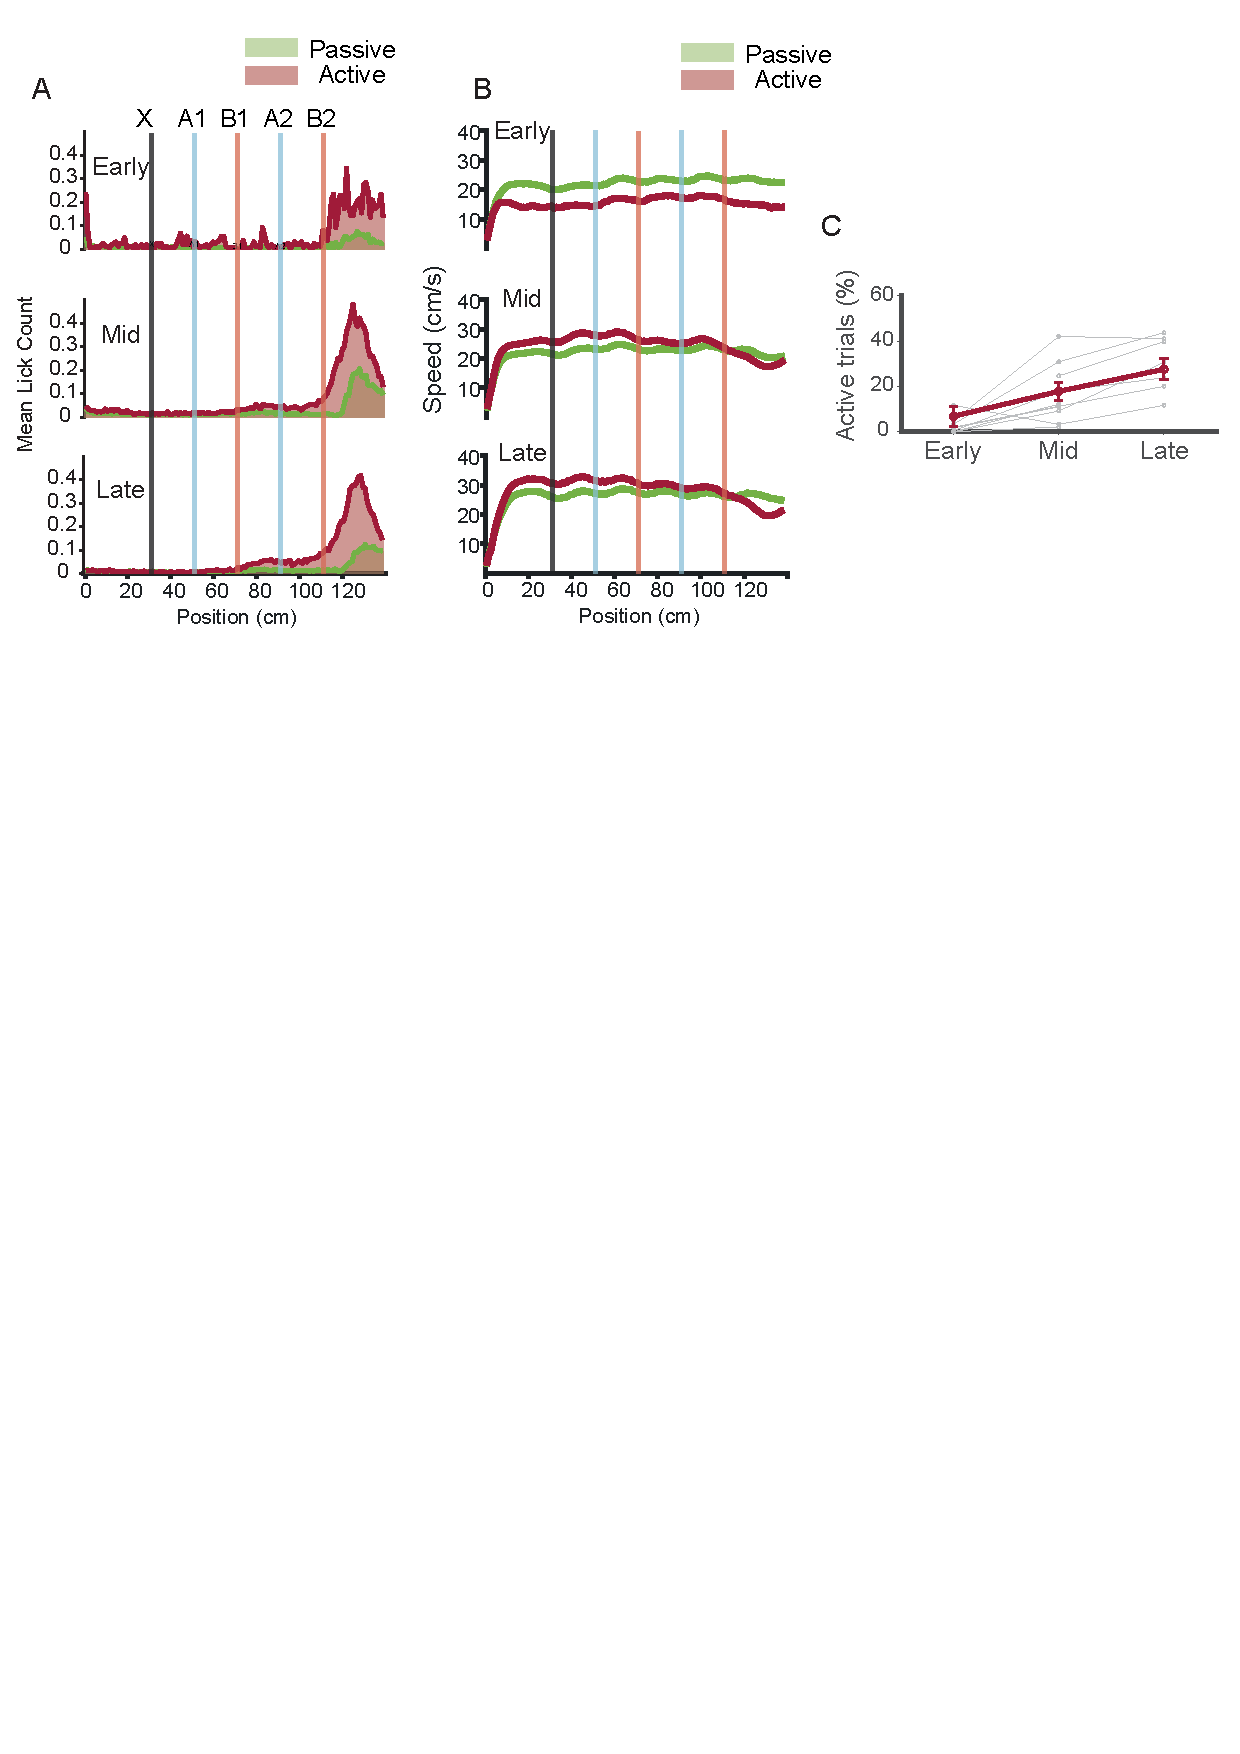
\includegraphics[width=1\linewidth]{figures//Chapter 3 Behaviour//Thesis Figures//figure_PDFs/fig3_behavioural_learning_summary.pdf}
    \caption{Behavioural Training Summary. }
\medskip
\small
Summaries of licking, running, and active reward rate across mice from early to late stage training. \textbf{A)} Average licking counts across mice from early to late training stages. Red is active reward trials and green is passive reward trials. \textbf{B)} Average running speed across mice along the VR corridor. Red is active reward trials and green is passive reward trials. \textbf{C)} Average active reward trial percentages from early to late stages and gray dots and lines are individual mice.
    \label{fig:training behaviour summary}
\end{figure}








\begin{figure}
    \centering
    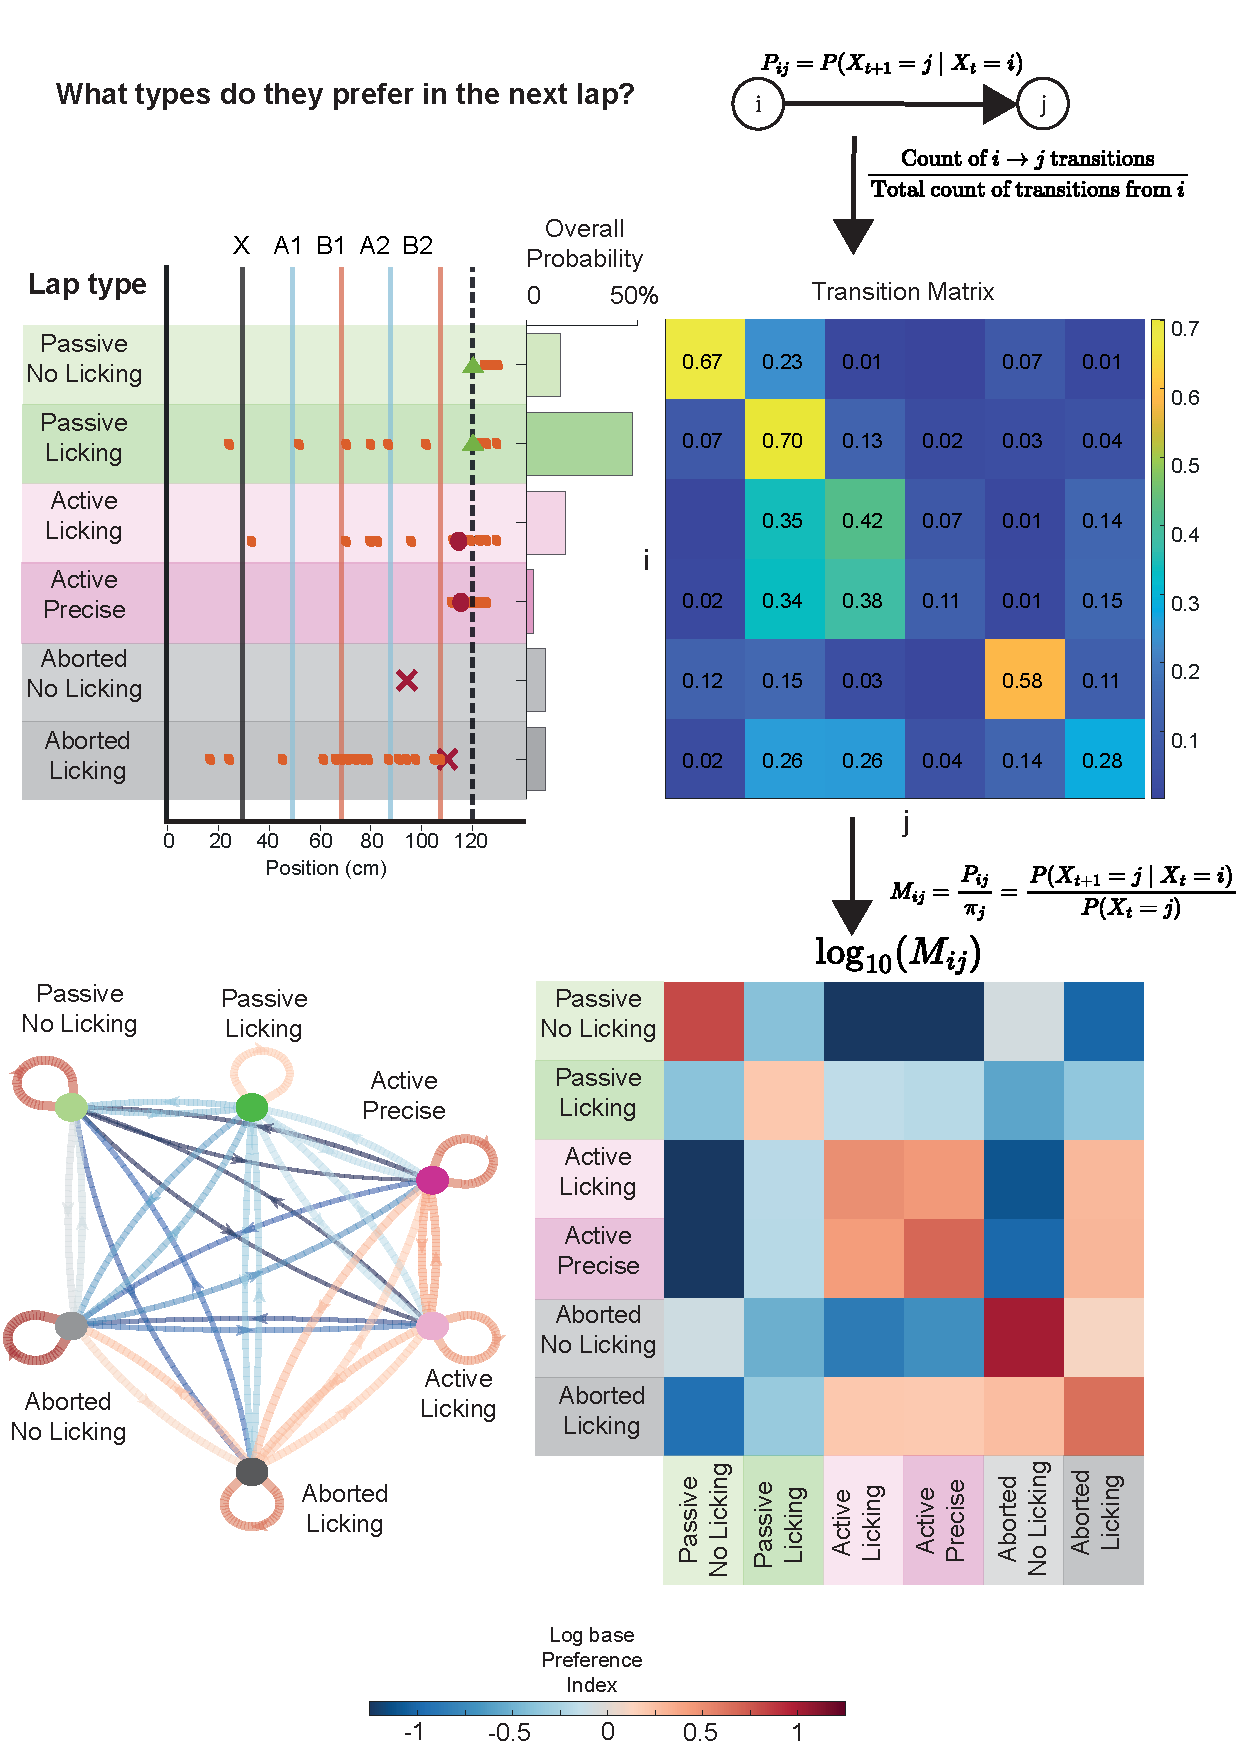
\includegraphics[width=1\linewidth]{figures//Chapter 3 Behaviour//Thesis Figures//figure_PDFs/fig4_transition_matrix.pdf}
    \caption{Laps of VR can be categorised into various types and they have preferences of which type to transition into.}

\medskip
\small
Demonstration of lap type categories, their transition matrix and their preference of transition which raises a question: when a lap type happens at lap i, does the animal prefer transitioning into a particular lap type at the next lap j? \textbf{A)} Each lap in the VR is categorised as one of six lap types. This panel demonstrates examples of each lap type and corresponding overall probability of lap type occuring next to the example. \textbf{B)} Illustration of how probabilities of transition state are calculated and an overall transition state matrix. \textbf{C)} Illustration of how to calculate preference index by dividing transition state probability over overall probability. Log likelihood of the preference can represent the direction of preferences well. On the left is the graph of the preference matrix and on the right is the preference matrix in log likelihood. 
    \label{fig:how to preference matrix}
\end{figure}






\begin{figure}
    \centering
    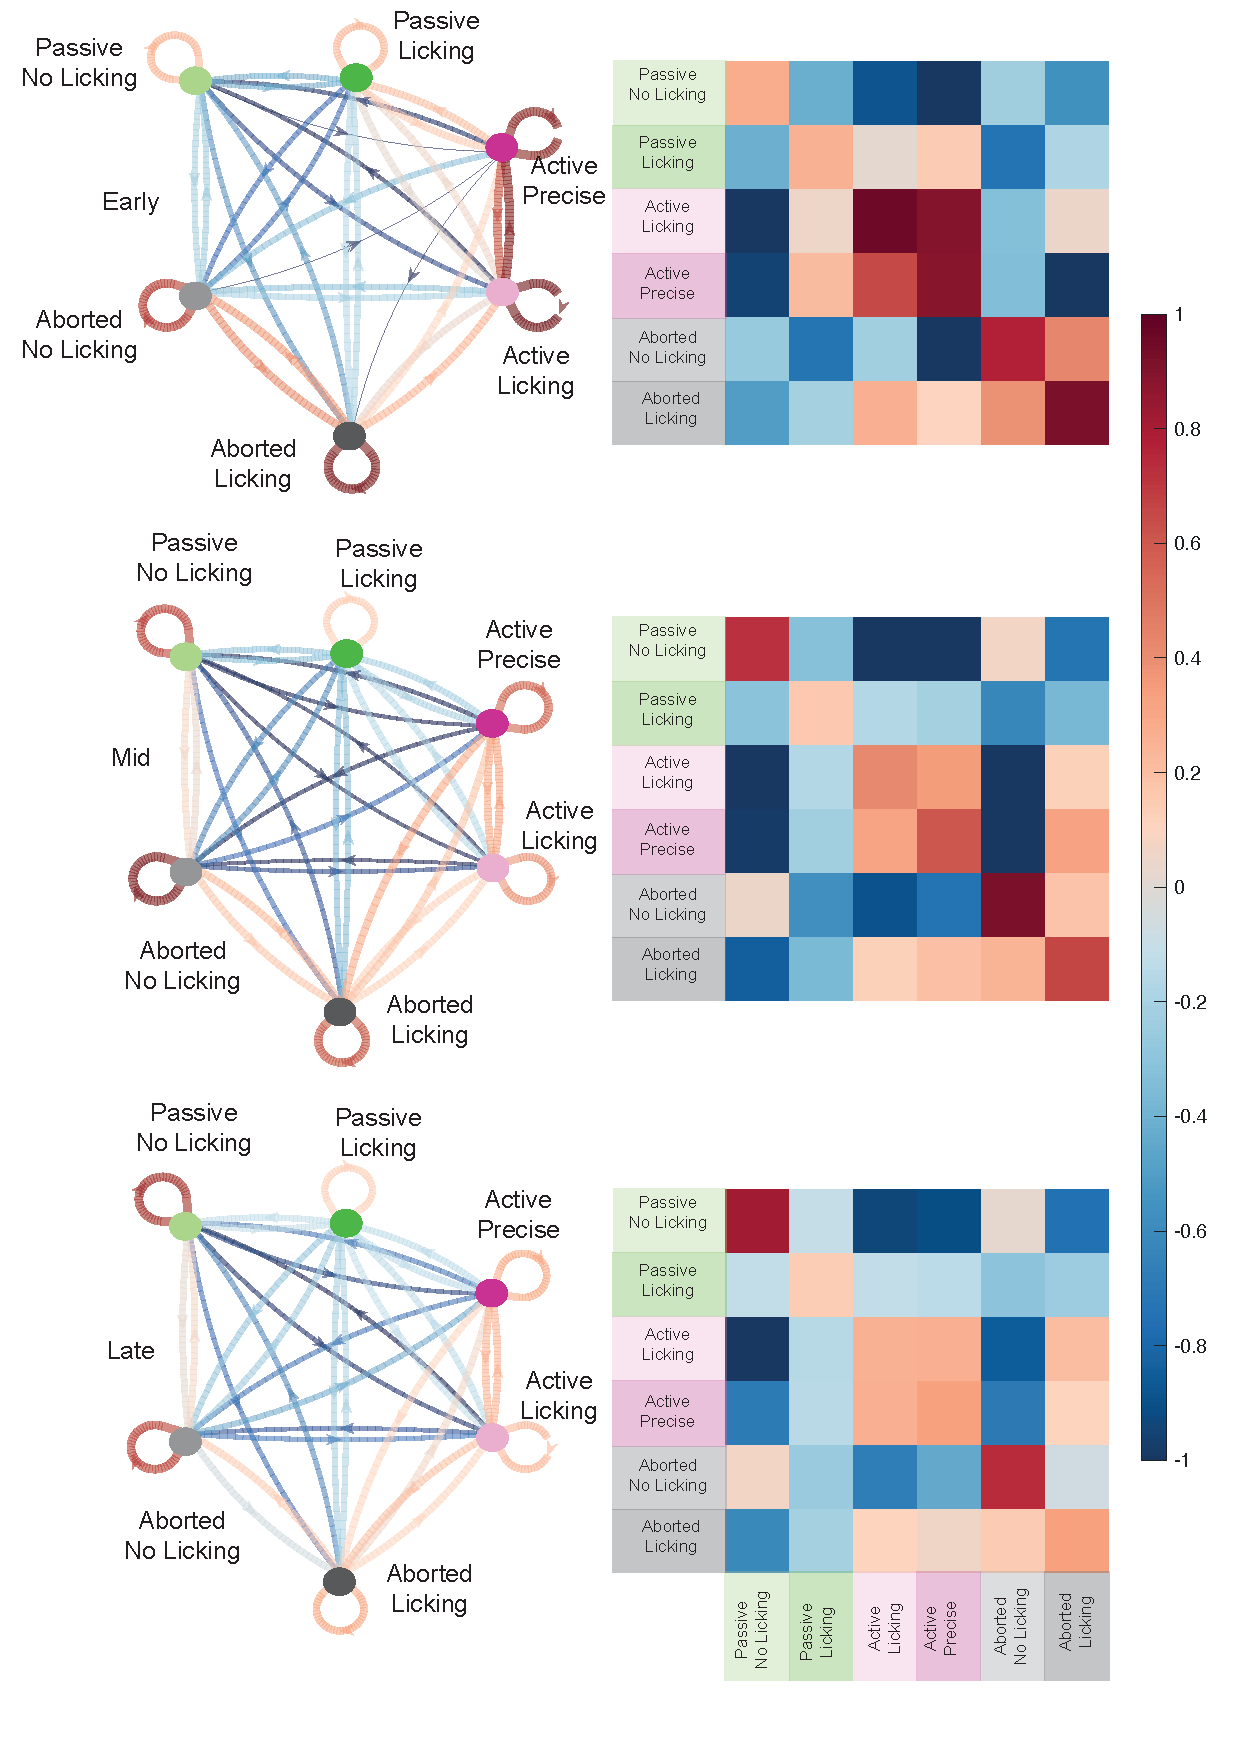
\includegraphics[width=1\linewidth]{figures//Chapter 3 Behaviour//Thesis Figures//figure_PDFs/fig5_preference_index_each_stage.pdf}
    \caption{Preference matrix for lap types over stages of training.}
\medskip
\small
Illustration of preference matrix over lap type at early, mid, and late stages of the training across mice. The preference matrix is presented as both graph and matrix itself for convenient interpretation.
    \label{fig:preference matrices over learning}
\end{figure}



\begin{figure}
    \centering
    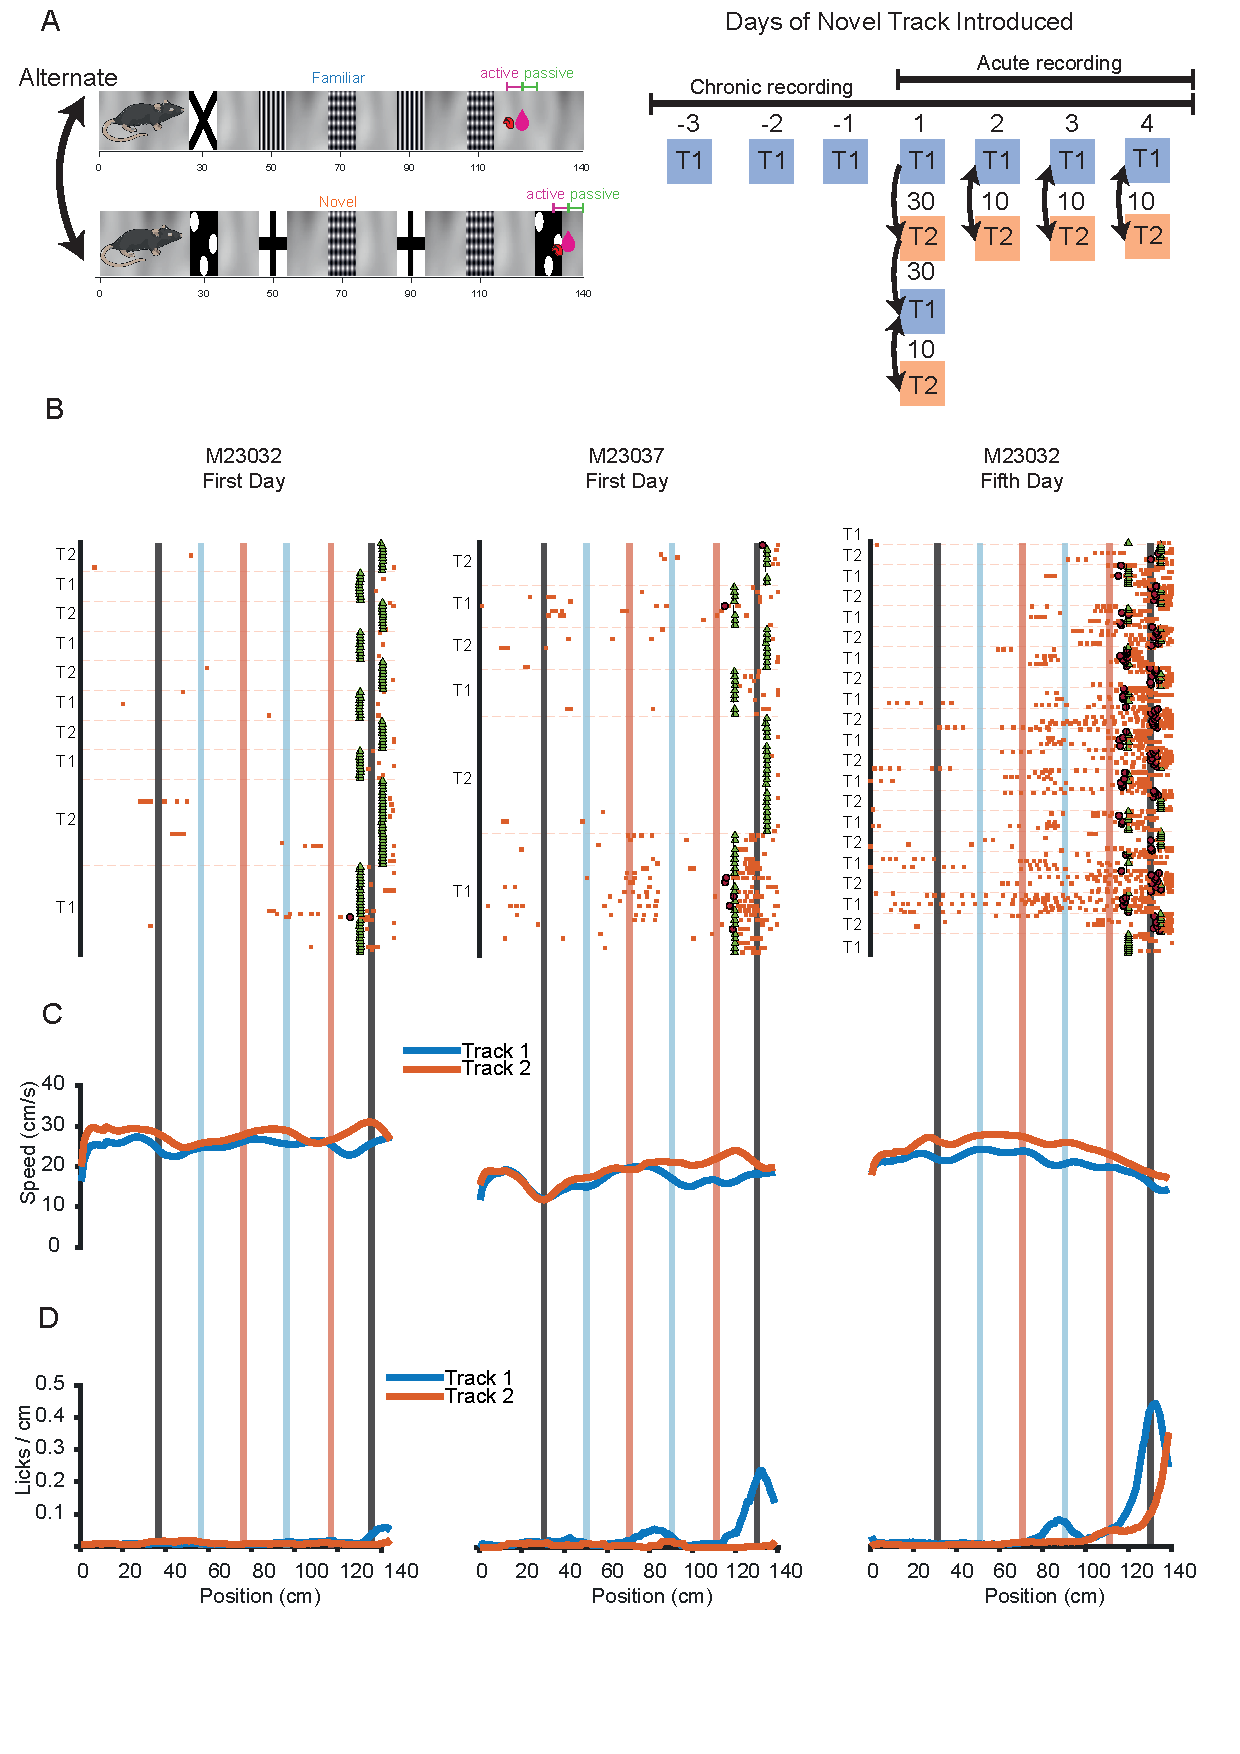
\includegraphics[width=1\linewidth]{figures//Chapter 3 Behaviour//Thesis Figures//figure_PDFs/fig6_novel_track_behaviour_examples.pdf}
    \caption{Mice adapt their behaviour when a novel environment is introduced.}

\medskip
\small
Examples of recording sessions behaviour when a novel environment is introduced. \textbf{A)} Demonstration of the experiment design and the timeline for when novel environment is introduced in recordings. \textbf{B)} Example raster plots of three sessions from recordings. Some sessions have poor active licking behaviour and the third example session shows high active licking behaviour in both environments. \textbf{C)} Average running speed in each session. Blue color is track 1 and red color is track 2. Track 2 is the novel environment. On average, the running behaviour is similar and much more different at the later part of the two environments. \textbf{D)}  Average lick count in each session. Track 1 is blue and track 2 is red orange. The licking distribution is different between the two tracks.  
    \label{fig:placeholder}
\end{figure}